Existem diversas ferramentas para se trabalhar com \LaTeX. Três ferramentas que merecem destaque são o editor \textit{Texmaker} (\autoref{fig:texmaker}), o ShareLaTeX (\autoref{fig:sharelatex}) e o gerenciador de referências \textit{JabRef} (\autoref{fig:jabref}). Todas as ferramentas são livres e multiplataforma. 

\begin{figure}[htb]
\caption{Tela do Texmaker}
 \label{fig:texmaker}
 \centering
 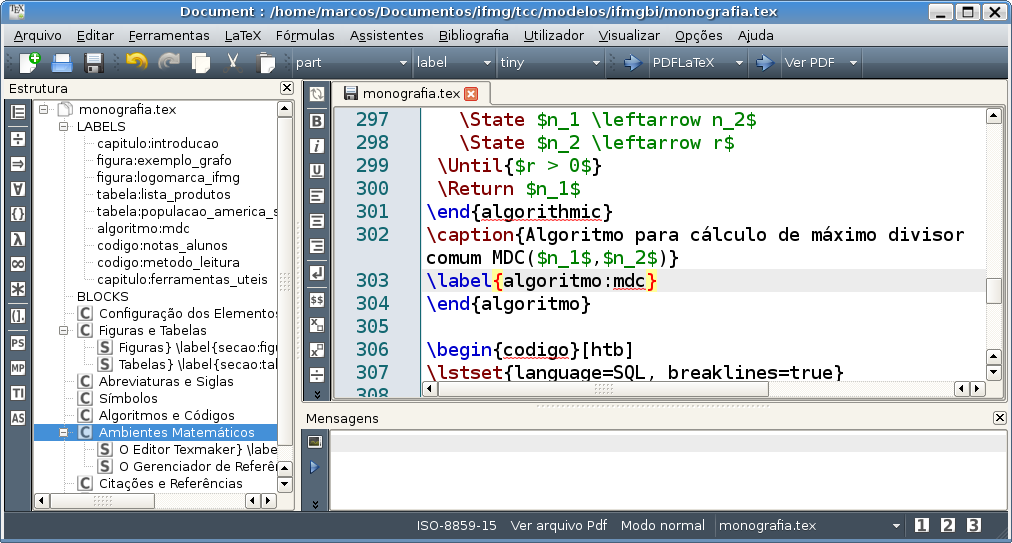
\includegraphics[width=\textwidth]{texmaker.png}
 \fautor
\end{figure}

\begin{figure}[htb]
\caption{Site do ShareLaTeX}
 \label{fig:sharelatex}
 \centering
 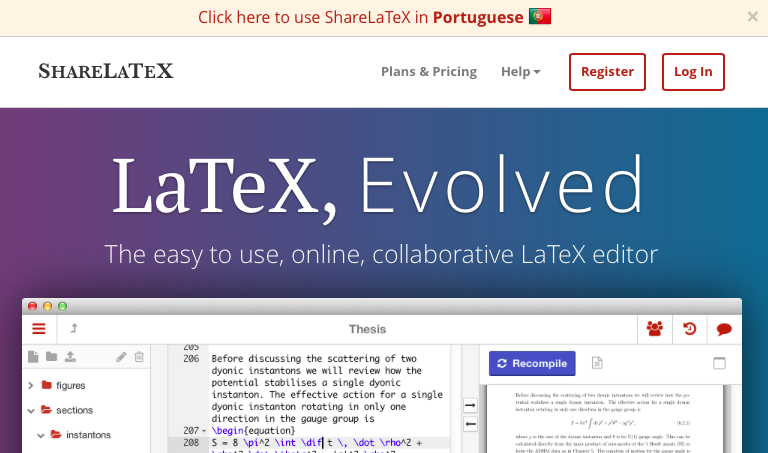
\includegraphics[scale=0.5]{sharelatex.png}
 \fautor
\end{figure}

\begin{figure}[htb]
 \caption{Tela do JabRef}
 \label{fig:jabref}
 \centering
 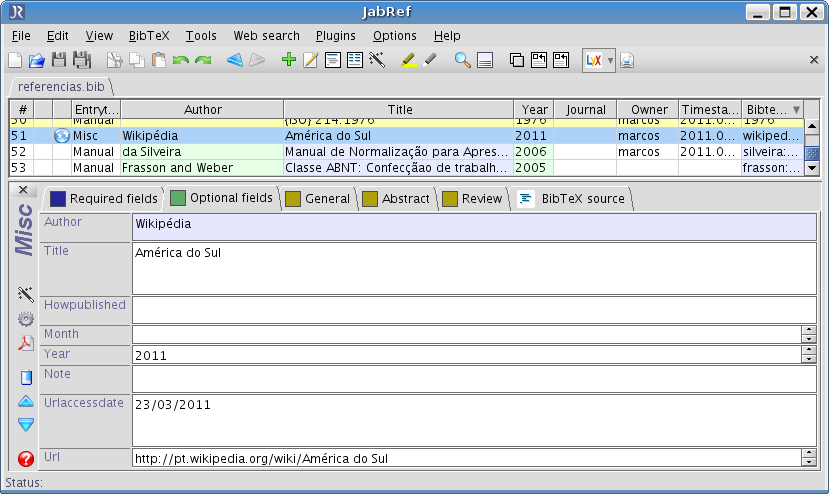
\includegraphics[scale=0.45]{jabref.png}
\fautor
\end{figure}

O Texmaker pode ser obtido em \url{www.xm1math.net/texmaker} e o JabRef pode ser obtido em \url{jabref.sourceforge.ne}. É importante ressaltar que o Texmaker é apenas um editor, para compilar os documentos é necessário um ambiente \LaTeX instalado. Os ambientes Latex mais populares são o Texlive (\url{www.tug.org/texlive}) e o MiKTex (\url{miktex.org}). 

As estrutura de referências do bibtex utilizadas nesse \textit{template} contém alguns parâmetros adicionais que o modelo geral não tem, conforme pode ser consultado em \citeonline{abntex2cite-alf}. Desta forma, recomenda-se fortemente o uso do gerenciador de referências JabRef, uma vez que é possível customizá-lo para atender estas exigências. O código de customização pode ser visto no \autoref{chapter:configuracao-jabref}.

O ShareLaTeX é uma ferramenta de edição de documento em \LaTeX de forma online e está disponível em \url{www.sharelatex.com}. A ferramenta permite o compartilhamento e edição simultânea do conteúdo. Além disso, pode-se consultar o histórico da edições realizadas no documento. A principal vantagem de utilizar o ShareLaTeX é não precisar instalar o compilador para LaTeX.